%% ut-thesis.tex -- document template for graduate theses at UofT
%%
%% Copyright (c) 1998-2012 Francois Pitt <fpitt@cs.utoronto.ca>
%% last updated at 09:43 (EDT) on Fri  1 Jun 2012
%%
%% This work may be distributed and/or modified under the conditions of
%% the LaTeX Project Public License, either version 1.3c of this license
%% or (at your option) any later version.
%% The latest version of this license is in
%%     http://www.latex-project.org/lppl.txt
%% and version 1.3c or later is part of all distributions of LaTeX
%% version 2005/12/01 or later.
%%
%% This work has the LPPL maintenance status "maintained".
%%
%% The Current Maintainer of this work is
%% Francois Pitt <fpitt@cs.utoronto.ca>.
%%
%% This work consists of the files listed in the accompanying README.

%% SUMMARY OF FEATURES:
%%
%% All environments, commands, and options provided by the `ut-thesis'
%% class will be described below, at the point where they should appear
%% in the document.  See the file `ut-thesis.cls' for more details.
%%
%% To explicitly set the pagestyle of any blank page inserted with
%% \cleardoublepage, use one of \clearemptydoublepage,
%% \clearplaindoublepage, \clearthesisdoublepage, or
%% \clearstandarddoublepage (to use the style currently in effect).
%%
%% For single-spaced quotes or quotations, use the `longquote' and
%% `longquotation' environments.


%%%%%%%%%%%%         PREAMBLE         %%%%%%%%%%%%

%%  - Default settings format a final copy (single-sided, normal
%%    margins, one-and-a-half-spaced with single-spaced notes).
%%  - For a rough copy (double-sided, normal margins, double-spaced,
%%    with the word "DRAFT" printed at each corner of every page), use
%%    the `draft' option.
%%  - The default global line spacing can be changed with one of the
%%    options `singlespaced', `onehalfspaced', or `doublespaced'.
%%  - Footnotes and marginal notes are all single-spaced by default, but
%%    can be made to have the same spacing as the rest of the document
%%    by using the option `standardspacednotes'.
%%  - The size of the margins can be changed with one of the options:
%%     . `narrowmargins' (1 1/4" left, 3/4" others),
%%     . `normalmargins' (1 1/4" left, 1" others),
%%     . `widemargins' (1 1/4" all),
%%     . `extrawidemargins' (1 1/2" all).
%%  - The pagestyle of "cleared" pages (empty pages inserted in
%%    two-sided documents to put the next page on the right-hand side)
%%    can be set with one of the options `cleardoublepagestyleempty',
%%    `cleardoublepagestyleplain', or `cleardoublepagestylestandard'.
%%  - Any other standard option for the `report' document class can be
%%    used to override the default or draft settings (such as `10pt',
%%    `11pt', `12pt'), and standard LaTeX packages can be used to
%%    further customize the layout and/or formatting of the document.

%% *** Add any desired options. ***
\documentclass[12pt]{ut-thesis}


%% *** Add \usepackage declarations here. ***
%% The standard packages `geometry' and `setspace' are already loaded by
%% `ut-thesis' -- see their documentation for details of the features
%% they provide.  In particular, you may use the \geometry command here
%% to adjust the margins if none of the ut-thesis options are suitable
%% (see the `geometry' package for details).  You may also use the
%% \setstretch command to set the line spacing to a value other than
%% single, one-and-a-half, or double spaced (see the `setspace' package
%% for details).

% some standard packages
\usepackage{times}
\usepackage{graphics}
\usepackage{graphicx}
\usepackage{caption}
\usepackage{subcaption}
% \usepackage{subfigure, epsfig}
\usepackage{float}
\usepackage{rotate}
\usepackage{amsmath}
\usepackage{amssymb}
\usepackage{mathtools}
\usepackage{dsfont}
\usepackage{bbm} % indicator function
\usepackage{tikz} % neural networks
\usetikzlibrary{matrix,chains,positioning,decorations.pathreplacing,arrows}
\usepackage{listings} % Include the listings-package
\usepackage{algorithm2e}


\setlength{\parskip}{3mm}

%%%%%%%%%%%%%%%%%%%%%%%%%%%%%%%%%%%%%%%%%%%%%%%%%%%%%%%%%%%%%%%%%%%%%%%%
%%                                                                    %%
%%                   ***   I M P O R T A N T   ***                    %%
%%                                                                    %%
%%  Fill in the following fields with the required information:       %%
%%   - \degree{...}       name of the degree obtained                 %%
%%   - \department{...}   name of the graduate department             %%
%%   - \gradyear{...}     year of graduation                          %%
%%   - \author{...}       name of the author                          %%
%%   - \title{...}        title of the thesis                         %%
%%%%%%%%%%%%%%%%%%%%%%%%%%%%%%%%%%%%%%%%%%%%%%%%%%%%%%%%%%%%%%%%%%%%%%%%

%% *** Change this example to appropriate values. ***
%\degree{Doctor of Philosophy}
\degree{Masters of Science}
%\department{Computer Science}
\department{Statistical Sciences}
\gradyear{2016}
\author{Mufan Li}
\title{Collaborative Filtering for Student Grade Analysis}

%% *** NOTE ***
%% Put here all other formatting commands that belong in the preamble.
%% In particular, you should put all of your \newcommand's,
%% \newenvironment's, \newtheorem's, etc. (in other words, all the
%% global definitions that you will need throughout your thesis) in a
%% separate file and use "\input{filename}" to input it here.

% convenient abbreviations
\newcommand{\de}{\partial}
\newcommand{\LL}{\mathcal{L}}
% \newcommand{\mb}{\mathbf}

% convenient abbreviations
\newcommand{\Cee}{\mathbf{C}}
\newcommand{\Iee}{\mathbf{I}}
\newcommand{\Lee}{\mathbf{L}}
\newcommand{\uD}{u_{\Delta}}
\newcommand{\mc}{\multicolumn}
\newcommand{\hs}{\hspace}
\newcommand{\EQ}{\begin{equation}}
\newcommand{\EN}{\end{equation}}
\newcommand{\EQA}{\begin{eqnarray}}
\newcommand{\ENA}{\end{eqnarray}}
\newcommand{\EQAS}{\begin{eqnarray*}}
\newcommand{\ENAS}{\end{eqnarray*}}

%% *** Adjust the following settings as desired. ***

%% List only down to subsections in the table of contents;
%% 0=chapter, 1=section, 2=subsection, 3=subsubsection, etc.
\setcounter{tocdepth}{2}

%% Make each page fill up the entire page.
\flushbottom


%%%%%%%%%%%%      MAIN  DOCUMENT      %%%%%%%%%%%%

\begin{document}

%% This sets the page style and numbering for preliminary sections.
\begin{preliminary}

%% This generates the title page from the information given above.
\maketitle
% \input{title}

%% There should be NOTHING between the title page and abstract.
%% However, if your document is two-sided and you want the abstract
%% _not_ to appear on the back of the title page, then uncomment the
%% following line.
%\cleardoublepage

%% This generates the abstract page, with the line spacing adjusted
%% according to SGS guidelines.
% \begin{abstract}
% %% *** Put your Abstract here. ***
% %% (At most 150 words for M.Sc. or 350 words for Ph.D.)
% This research project applied machine learning 
% to analyze the student grade dataset from \cite{BaRoYo14},
% which contains complete transcripts of undergraduate students
% from a major Canadian University.
% Specifically, neural network methods 
% are used to predict student selections of courses and 
% majors, as well as the grade performance in 
% future courses.
% % \input{abstract}

% \end{abstract}

%% Anything placed between the abstract and table of contents will
%% appear on a separate page since the abstract ends with \newpage and
%% the table of contents starts with \clearpage.  Use \cleardoublepage
%% for anything that you want to appear on a right-hand page.

%% This generates a "dedication" section, if needed
%% (uncomment to have it appear in the document).
%\begin{dedication}
%%% *** Put your Dedication here. ***
%Put your Dedication here.
%\end{dedication}

%% The `dedication' and `acknowledgements' sections do not create new
%% pages so if you want the two sections to appear on separate pages,
%% you should put an explicit \newpage between them.

% \newpage
%% This generates an "acknowledgements" section, if needed
%% (uncomment to have it appear in the document).
% \begin{acknowledgements}
% %% *** Put your Acknowledgements here. ***
% I have to thank my advisor Professor Jeffrey Rosenthal and 
% Professor Albert Hyoon,
% without their careful guidance this research project would not have been possible.
% Under Professor Christara's supervision,
% this research project has been an amazing learning experience.
% I would like to thank you very much for your support and teaching over the 
% past year.
% \end{acknowledgements}

%% This generates the Table of Contents (on a separate page).
\tableofcontents

%% This generates the List of Tables (on a separate page), if needed
%% (uncomment to have it appear in the document).
\listoftables

%% This generates the List of Figures (on a separate page), if needed
%% (uncomment to have it appear in the document).
\listoffigures

%% You can add commands here to generate any other material that belongs
%% in the head matter (for example, List of Plates, Index of Symbols, or
%% List of Appendices).

%---------------------------------------------------
% need list of symbols
%---------------------------------------------------

%% End of the preliminary sections: reset page style and numbering.
\end{preliminary}


%%%%%%%%%%%%%%%%%%%%%%%%%%%%%%%%%%%%%%%%%%%%%%%%%%%%%%%%%%%%%%%%%%%%%%%%
%%  Put your Chapters here; the easiest way to do this is to keep     %%
%%  each chapter in a separate file and `\include' all the files.     %%
%%  Each chapter file should start with "\chapter{ChapterName}".      %%
%%  Note that using `\include' instead of `\input' will make each     %%
%%  chapter start on a new page, and allow you to format only parts   %%
%%  of your thesis at a time by using `\includeonly'.                 %%
%%%%%%%%%%%%%%%%%%%%%%%%%%%%%%%%%%%%%%%%%%%%%%%%%%%%%%%%%%%%%%%%%%%%%%%%

%% *** Include chapter files here. ***

% Introduction

\chapter{Introduction} \label{sc:intro}

\paragraph{}
Recent developments in machine learning have made significant 
contributions to a wide range of fields that are not 
traditionally considered data science.
% Notably the Netflix competition have attracted a collective
% effort in developing models that greatly improved prediction
% of movie ratings by different users,
% creating the best movie recommendation system at the time \cite{FeHeKh12}.
% Similar to the Netflix rating data,
% student grades in different courses follow the same structure,
% allowing the application of the same machine learning techniques.
In this research course, we intend to explore several of the 
machine learning techniques in applications to education.

\paragraph{}
Specifically, this research project aims to apply machine learning 
to analyze the student grade dataset from \cite{BaRoYo14},
which contains complete transcripts of undergraduate students
from a major Canadian University.
Similar to predicting user ratings,
we are able to predict the grades for courses.
From the predictions, this project intends to analyze
the effect of choosing easier courses on student grades,
specifically by comparing the predicted grades of courses
students did not take against the courses taken 
within the same program.
By analyzing the variation in course difficulty,
these results could potentially improve curriculum design 
for educational institutions and admission procedure for
graduate programs.

\paragraph{}
The project will focus on implementing three main methods of inference:
\vspace{-0em}
\begin{enumerate}
\setlength\itemsep{-0.2em}
  \item Matrix factorization (MF) \cite{FeHeKh12} and if time permits
  	probabilistic matrix factorization (PMF) \cite{MnSa07, SaMn08}
  \item Restricted Boltzmann machines (RBM) \cite{Sa09}
  \item Denoising auto-encoders (DAE) \cite{VLLBM10} and if time permits
  	variational auto-encoders (VAE) \cite{KiWe13}
\end{enumerate}



% 2. Background

\chapter{Background} \label{ch:background}

\section{Supervised Learning Using Feedforward Neural Networks} \label{sc:nnet}

\paragraph{}
We first consider a class of machine learning algorithms
called supervised learning. 
In this case we have a dataset $\mathcal{D} = \{\mathbf{x}^{[n]}, 
\mathbf{y}^{[n]}\}, \mathbf{x}^{[n]} \in \mathbb{R}^{N_{in}}, 
\mathbf{y}^{[n]} \in \mathbb{R}^{N_{out}}, n \in \mathbb{N}$,
with $\mathbf{x}$ as the input, and $\mathbf{y}$ as the label or output.
We want to find a model 
$f(\mathbf{x},\mathbf{w})$ such that 
it is the ``closest'' to $\mathbf{y}$, 
with $\mathbf{w}$ the parameters in the model.
This section will introduce neural networks as the model $f$
that predicts the labels $\mathbf{y}$.

In the simplest case, neural networks can be reduced to 
a generalized linear model (GLM),
where the prediction is a linear combination of inputs
but passed through a non-linear function:
%
\begin{equation}
	f(\mathbf{x},\mathbf{w}) = g\left( \sum_{i=1}^{N_{in}} w_i x_i + w_0 \right)
\end{equation}
%
\indent Here $g(\cdot)$ is a non-linear function, 
with $\mathbf{x}$ is an $N$ dimensional input vector,
and $\mathbf{w}$ is the weight vector,
which includes $w_0$ as the bias.
Common choices of $g(\cdot)$, also known as activation functions,
for neural networks 
include the logistic (sigmoid) function, the hyperbolic tangent function, 
and the rectified linear unit (ReLU):
%
\begin{equation}
\begin{aligned}
	g_{\text{logistic}}(z) &= \frac{1}{1+e^{-z}} \\
	g_{\text{tanh}}(z) &= \tanh(z) = \frac{1 - e^{-2z}}{1 + e^{-2z}}\\
	g_\text{ReLU}(z) &= \max(z,0)
\end{aligned}
\end{equation}
%
% \indent 
where $z = \left( \sum_{i=1}^N w_i x_i + w_0 \right)$ 
denotes the linear combination for GLMs.
Notice all of these functions have simple derivatives,
and specifically logistic and hyperbolic tangent functions 
are monotonic and bounded by their horizontal asymptotes at infinities,
which makes them great choices for binary classification problems.

Graphically, this can be represented by a series of 
input nodes $\{x_i\}$ connected to an output node $f$,
with weights $\{w_i\}$ on the connections.
Note bias is omitted from the graph but remains a parameter.

\def\layersep{2.5cm}
\begin{figure}[h]
\centering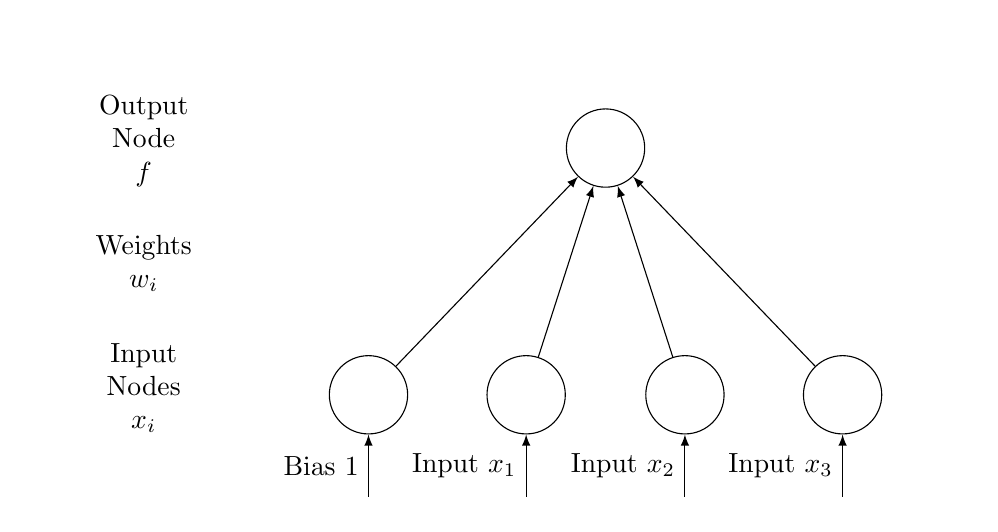
\begin{tikzpicture}[
plain/.style={
  draw=none,
  fill=none,
  },
net/.style={
  matrix of nodes,
  nodes={
    draw,
    circle,
    inner sep=10pt
    },
  nodes in empty cells,
  column sep=0pt,
  row sep=-1cm
  },
>=latex
]

\matrix[net] (mat)
{
|[plain]| \parbox{1.2cm}{\centering Output Node\\$f$} & |[plain]| & 
    |[plain]| & |[plain]| & |[plain]| & & |[plain]| & |[plain]| & |[plain]| 
    & |[plain]| \\
|[plain]| \parbox{1.3cm}{\centering Weights\\$w_{i}$}
    &|[plain]| &|[plain]| &|[plain]| &|[plain]| &
    |[plain]| &|[plain]| &|[plain]| &|[plain]| &|[plain]| \\
|[plain]| \parbox{1.3cm}{\centering Input Nodes\\$x_i$} & 
    |[plain]| & & |[plain]| & & |[plain]| & & |[plain]| &\\
};
\foreach \ai [count=\mi ]in {5,7,9}
  \draw[<-] (mat-3-\ai) -- node[left] {Input $x_\text{\mi}$} +(0cm,-1.3);
\draw[<-] (mat-3-3) -- node[left] {Bias 1} +(0cm,-1.3);
\foreach \ai in {6}
{\foreach \aii in {3,5,7,9}
  \draw[<-] (mat-1-\ai) -- (mat-3-\aii);
}
\end{tikzpicture}

\caption{\label{fig:GLM}
A generalized linear model represented in graphical form.
In a neural network, this is also referred to as a single neuron.
}
\end{figure}

%formatting
% \pagebreak

A general feed-forward neural network is defined by recursive GLMs
with different weights.
For example, a neural network with two hidden layers
(three layers of recursion) is defined as:
%
\begin{equation}
\begin{aligned}
	h^{(1)}_j &= g^{(1)}
		\left(\sum_{i=1}^{N^{(1)}} w_{ij}^{(1)} x_i + 
      w^{(1)}_{0j} \right) \\
	h^{(2)}_k &= g^{(2)}
		\left(\sum_{j=1}^{N^{(2)}} w_{jk}^{(2)} h_j^{(1)} + 
      w^{(2)}_{0k} \right) \\
	f_l &= g^{(3)}
		\left(\sum_{k=1}^{N^{(3)}} w_{kl}^{(3)} h_k^{(2)} + 
      w^{(3)}_{0l} \right)
\end{aligned}
\end{equation}
%
where $g(\cdot)^{(\alpha)}$ is some activation function,
$h^{(\alpha)}_j$ denotes the $j^\text{th}$ node of the $\alpha^\text{th}$ 
hidden layer,
$w_{ij}^{(\alpha)}$ denotes the weight for the connection of 
the $i^\text{th}$ node of the $\alpha^\text{th}$ layer to 
the $j^\text{th}$ node of the $(\alpha+1)^\text{th}$ layer,
and $N^{(\alpha)}$ denotes the number of nodes in the $\alpha^\text{th}$ layer.
Additionally, let $N^{(4)}$ be the number of 
output nodes $f_l$,
and $\mathbf{w} = \left[\mathbf{w}^{(1)} \mathbf{w}^{(2)} \mathbf{w}^{(3)} \right]$.
Here we also note that $N^{(1)}$ is the number of input nodes.

Graphically, this structure has a very clear representation:
%
\def\layersep{2.5cm}
\begin{figure}[h]
\centering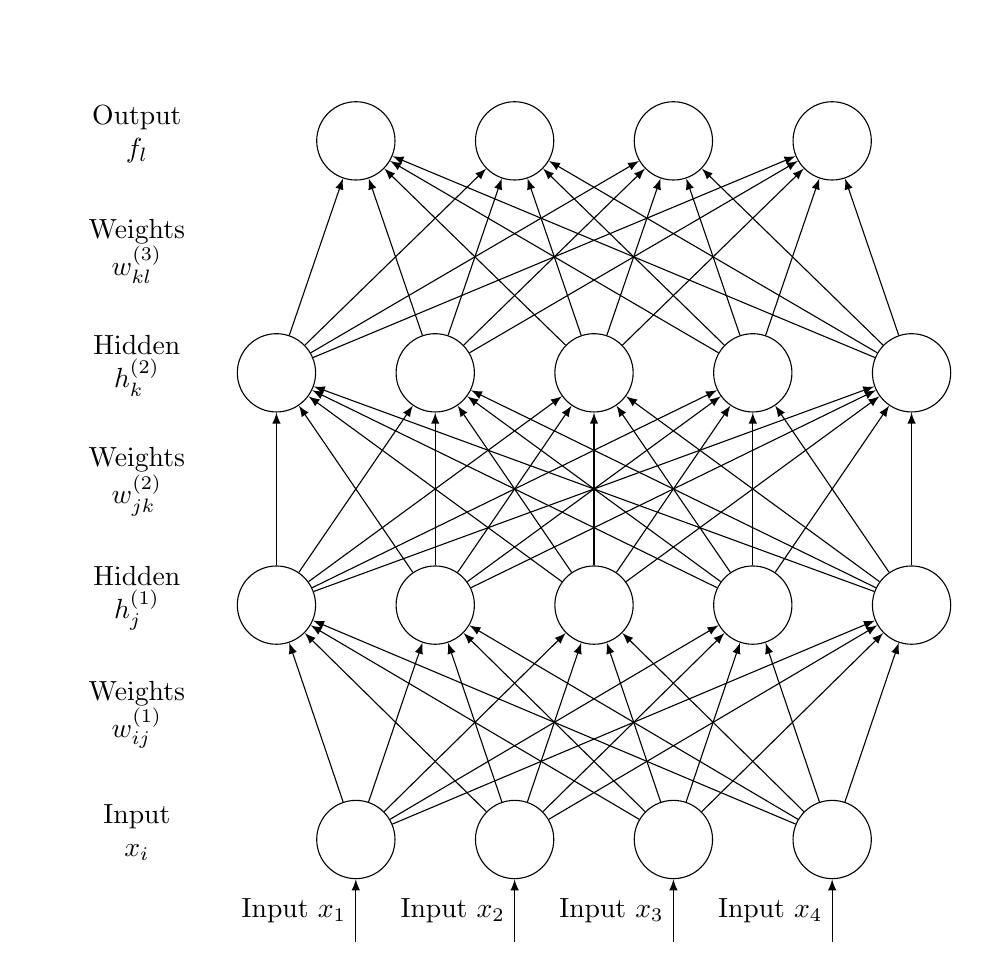
\begin{tikzpicture}[
plain/.style={
  draw=none,
  fill=none,
  },
net/.style={
  matrix of nodes,
  nodes={
    draw,
    circle,
    inner sep=10pt
    },
  nodes in empty cells,
  column sep=0pt,
  row sep=-1cm
  },
>=latex
]

\matrix[net] (mat)
{
|[plain]| \parbox{1.3cm}{\centering Output\\$f_l$} & 
    |[plain]| & & |[plain]| & & |[plain]| & & |[plain]| &\\
|[plain]| \parbox{1.3cm}{\centering Weights \\$w_{kl}^{(3)}$}\\
    % &|[plain]| &|[plain]| &|[plain]| &|[plain]| &
    % |[plain]| &|[plain]| &|[plain]| &|[plain]| &|[plain]| \\
|[plain]| \parbox{1.2cm}{\centering Hidden\\$h_k^{(2)}$} & & 
    |[plain]| & & |[plain]| & & |[plain]| & & |[plain]| & \\
|[plain]| \parbox{1.3cm}{\centering Weights \\$w_{jk}^{(2)}$}
    &|[plain]| &|[plain]| &|[plain]| &|[plain]| &
    |[plain]| &|[plain]| &|[plain]| &|[plain]| &|[plain]| \\
|[plain]| \parbox{1.2cm}{\centering Hidden\\$h_j^{(1)}$} & & 
    |[plain]| & & |[plain]| & & |[plain]| & & |[plain]| & \\
|[plain]| \parbox{1.3cm}{\centering Weights \\$w_{ij}^{(1)}$}
    &|[plain]| &|[plain]| &|[plain]| &|[plain]| &
    |[plain]| &|[plain]| &|[plain]| &|[plain]| &|[plain]| \\
|[plain]| \parbox{1.3cm}{\centering Input\\$x_i$} & 
    |[plain]| & & |[plain]| & & |[plain]| & & |[plain]| &\\
};
\foreach \ai [count=\mi ]in {3,5,7,9}
  \draw[<-] (mat-7-\ai) -- node[left] {Input $x_\text{\mi}$} +(0cm,-1.3);
\foreach \ai in {3,5,7,9}
{\foreach \aii in {2,4,...,10}
  \draw[<-] (mat-1-\ai) -- (mat-3-\aii);
}
\foreach \ai in {2,4,...,10}
{\foreach \aii in {2,4,...,10}
  \draw[<-] (mat-3-\ai) -- (mat-5-\aii);
}
\foreach \ai in {2,4,...,10}
{\foreach \aii in {3,5,7,9}
  \draw[<-] (mat-5-\ai) -- (mat-7-\aii);
}
\end{tikzpicture}

\caption{\label{fig:NN}
A generalized feed-forward neural network with two hidden layers. 
Bias parameters are not drawn for compactness, 
although they are present in all forward passing nodes.
}
\end{figure}

% formatting
% \pagebreak 

While most GLMs do not admit a closed-form solution,
a satisfactory optimization can be achieved by the gradient descent method.
In the neural network case,
the optimization becomes more difficult as
the number of parameters increase with the number of nodes and layers.
However, we can still apply the gradient descent method
and find a local optimum for the simpler neural networks. \cite{Bi07}

Once again we have a dataset $\mathcal{D} = \{\mathbf{x}^{[n]}, 
\mathbf{y}^{[n]}\}, n \in \mathbb{N}$,
and we want to find a model $f(\mathbf{x},\mathbf{w})$ such that 
it is the ``closest'' to $\mathbf{y}$.
If the error function $E(f,\mathbf{y})$
and the model $f(\mathbf{x},\mathbf{w})$ are differentiable
with respect to $\mathbf{w}$,
the model can be optimized by gradient descent.
In other words, for any randomly initialized $\mathbf{w}^0$,
an improvement $\mathbf{w}^{k+1}$ can be obtained by making a 
small modification
in the direction of the gradient with respect to $\mathbf{w}^k$ :
%
\begin{equation}
	\mathbf{w}^{k+1} = \mathbf{w}^{k} - \eta \; \nabla_{\mathbf{w}^k} 
					E\left(f(\mathbf{x},\mathbf{w}^k),\mathbf{y}\right)
\end{equation}
%
where $\eta > 0$ is hyper-parameter controlling the change of 
each optimization iteration, commonly called the learning rate.
Note $\eta$ is not part of the final model $f(\mathbf{x},\mathbf{w})$,
but it will significantly influence optimization.

In the two hidden layer neural network previously,
a derivative with respect to any weight 
$w_{ij}^{(\alpha)}$ can be found
by applying the chain rule to the derivatives.
For example the derivative with respect to $w_{jk}^{(2)}$ 
where $j \neq 0$ :
%
\begin{equation}
\begin{aligned}
	\text{let } z_j^{(\alpha)} &= 
		\sum_{i=1}^{N^{(\alpha)}} w_{ij}^{(\alpha)} h_i^{(\alpha-1)}
      + w_{0j}^{(\alpha)} \\
	\text{then } \frac{\de E}{\de w_{jk}^{(2)}} &= 
		\sum_{l=1}^{N^{(4)}} \frac{\de E}{\de f_l}
		\frac{\de f_l}{\de z_l^{(3)}}
		\frac{\de z_l^{(3)}}{\de h_k^{(2)}}
		\frac{\de h_k^{(2)}}{\de z_k^{(2)}}
		\frac{\de z_k^{(2)}}{\de w_{jk}^{(2)}} \\
	&=
		\sum_{l=1}^{N^{(4)}} \frac{\de E}{\de f_l}
		\frac{\de g^{(3)}(z_l^{(3)}) } {\de z_l^{(3)}}
		w_{kl}^{(3)}
		\frac{\de g^{(2)}(z_k^{(2)}) } {\de z_k^{(2)}}
		h_j^{(1)} .
\end{aligned}
\end{equation}
%
% \indent 
Recall $g^{(\alpha)}(\cdot)$ is selected to have a simple derivative,
making the complex appearing gradient term above easy to compute.

A common technique to improve speed of convergence 
is by adding momentum.
Instead of letting the gradient dictate the change in $\mathbf{w}^k$,
the idea is to let the gradient dictate the rate of change.
If $\mathbf{w}^k$ is interpreted as a coordinate,
and each optimization iteration as velocity,
momentum can be seen as using the gradient as acceleration
instead of velocity. 
This allows the optimization to accumulate speed in 
a consistent direction of the gradient, 
while making it harder to slow down and 
converge to a poor local minimum.
The formulation starts with a velocity vector $\mathbf{v}^0$
initialized to zero, and the rest in similar:
%
\begin{equation}
\begin{aligned}
	\mathbf{v}^{k+1} &= \theta \mathbf{v}^{k} - \eta \; \nabla_{\mathbf{w}^k} 
				E\left(f(\mathbf{x},\mathbf{w}^k),\mathbf{y}\right) \\
	\mathbf{w}^{k+1} &= \mathbf{w}^{k} + \mathbf{v}^{k+1}
\end{aligned}
\end{equation}
%
where $\theta \in [0,1]$ is the hyper-parameter 
deciding the preservation of momentum.
Here choosing a larger $\theta$ would result in a stronger 
preservation of the velocity vector $\mathbf{v}$,
which then retains more momentum.

% % formatting
% \pagebreak
% \noindent
% \large
% {\bf MNIST Hand-Written Digits}
% \normalsize













\section{MNIST Hand-Written Digits Example} \label{sc:MNIST}

\paragraph{}
The Mixed National Institute of Standards and Technology
(MNIST) dataset \cite{Le98} is a collection of images of hand-written digits
from various sources,
with each image labeled the correct digit.
The dataset contains 60,000 images for training (fitting),
and 10,000 images for testing.
The images are 28x28 in resolution,
hence making $N^{(1)} = 784$ dimensions in input.

The data labels are changed to use the 1-of-K encoding scheme,
where the label $\mathbf{y}$ is a binary vector of size K,
with only one element taking a value of one.
In this case, given 10 possible digits,
we have a vector of size $N^{(4)} = 10$.
For example, a possible scheme can label the digit ``$3$'' 
using the vector $[0,0,1,0,\ldots]$ where 
only the $3^\text{rd}$ index is a ``$1$''.

To best model this type of label vector,
the softmax function is chosen for the output layer:
%
\begin{equation}
	f_l = 
	g^{(3)}(z_l^{(3)}) = \frac{\exp(z_l^{(3)})}
		{\sum_{k=1}^{N^{(4)}} \exp(z_k^{(3)})}
\end{equation}
%
where $z^{(3)}_l = \sum_{k=1}^{N^{(3)}} w_{kl}^{(3)} h_k^{(2)} + 
      w^{(3)}_{0l}$ 
      is a linear combination of the final hidden layer.
Since the denominator normalizes the sum, the $f_l$ now adds up to one,
and a ``perfect'' output is exactly the 1-of-K encoded label.
If $f_l$ is modeled as the probability of the image being digit $l$,
suppose the correct digit is $m$,
then the likelihood of making the correct prediction is:
%
\begin{equation}
  L(\mathbf{f},\mathbf{y}) = f_m = \prod_{l=1}^{N^{(4)}} f_l \, ^{y_l}
\end{equation}
%
since $y_m = 1$ is the only non-zero term in the label vector.
We can then define the error function as negative log-likelihood:
%
\begin{equation}
% \begin{aligned}
	E(\mathbf{f},\mathbf{y}) 
		= - \log \prod_{l=1}^{N^{(4)}} f_l \, ^{y_l}
		= - \sum_{l=1}^{N^{(4)}} y_l \log f_l
% \end{aligned}
\end{equation}
%
where $N^{(4)}$ is the number of output nodes, 
and minimizing $E$ is equivalent to maximizing likelihood.
Note taking the logarithm creates an error function with much
simpler derivative, 
hence simplifying the gradient descent method.

In the following experiment, 
a two hidden layer neural network is used to model the MNIST digits.
We used $N^{(2)} = N^{(3)} = 1000$ nodes in the hidden layers, 
creating a structure of 784-1000-1000-10 
$\left( N^{(1)} - N^{(2)} - N^{(3)} - N^{(4)} \right)$
nodes in each layer.
We also chose 
$g^{(1)}(\cdot) = g^{(2)}(\cdot) = g_\text{ReLU}(\cdot)$ 
in the hidden layers,
and softmax for the output layer.
The hyper parameters were chosen as $\eta = 10^{-5}$
and $\theta = 0.9$.
We also chose to update the weight vector $\mathbf{w}^k$ once
for every 100 samples of digits,
also known as a mini-batch.

After training (optimizing) for 50 epochs,
with each epoch denoting one complete run through of the training 
dataset,
we reach a test error rate of $16\%$ (Figure \ref{fig:mnist_err}).
%
\begin{figure}[h]
\centering
\begin{subfigure}{.45\textwidth}
  \centering
  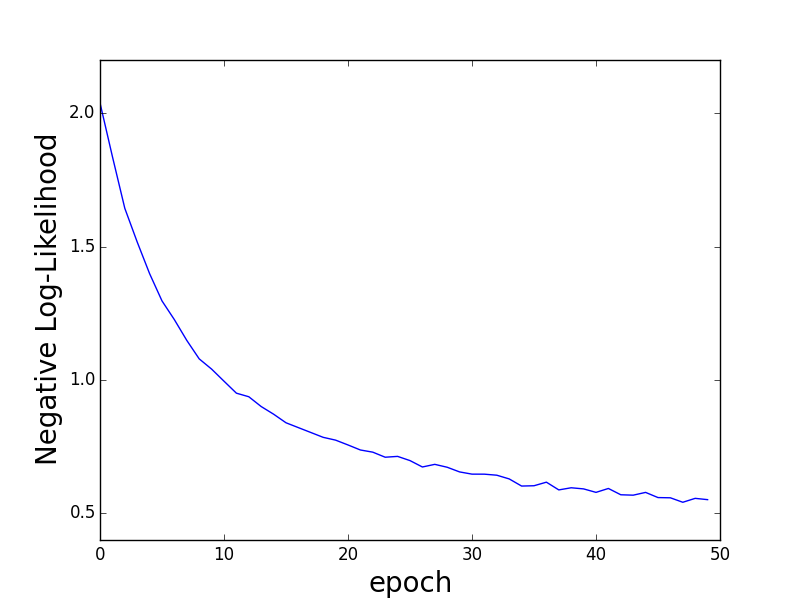
\includegraphics[width=\linewidth]{fig_mnist_nll.png}
  \caption{The negative log-likelihood}
  \label{fig:mnist_nll}
\end{subfigure}%
\begin{subfigure}{.45\textwidth}
  \centering
  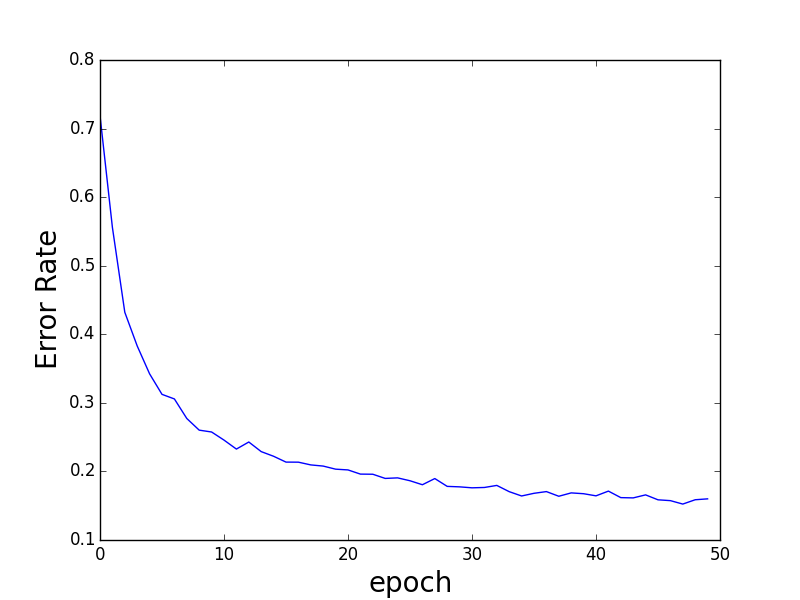
\includegraphics[width=\linewidth]{fig_mnist_err.png}
  \caption{The classification error rate}
  \label{fig:mnist_err}
\end{subfigure}
\caption{MNIST hand-written digits modeled using a two hidden
  layer neural network, with negative log-likelihood and
  classification error rate computed after each epoch.}
\label{fig:mnist_results}
\end{figure}
%
By increasing the number of epochs and a few minor modifications,
this model could potentially reach error rates as low as $2\%$.
However, this will not be explored since it is not
the main purpose of this document,
and optimization can be very time consuming due to computation.

% It is important to note that the activation function chosen is ReLU, 
% which is not easy to incorporate due within a 
% restricted Boltzmann machine context due to an unbounded range.
% However, a recently introduced method called 
% general adversarial networks can be used instead using the ReLU functions
% in alternative to restricted Boltzmann machines.
% This will be explored further in future discussions.

While the technique is more than a sufficient solution 
for recognizing hand-written digits,
naively applying gradient descent to more complex 
neural networks tend to have poor results.
Alternative methods will be discussed in the next section 
in order to address this problem.

Also note this type of neural networks is feed-forward, 
which mean it is limited to only supervised type problems
where the data structure is consistent 
and a prediction target (label) is provided for each sample.
For a collaborative filtering type problem,
the inference is often made within the data structure itself, 
which makes an unsupervised learning problem.
Feed-forward neural networks also fail to fully utilize 
the datasets that are partly labeled, 
known as semi-supervised problems.
These problems would require other variations of neural networks
with different methods for inference.

















\section{Restricted Boltzmann Machines} \label{sc:rbm}

\paragraph{}
On the other hand, restricted Boltzmann machines (RBM) is a
completely different approach to problems without labels.
RBM is a type of unsupervised learning algorithm, 
for there are no labels to ``supervise'' the learning.
The purpose of unsupervised algorithms are to find
structural patterns within the data itself.
In this case, we are interested in the relationships 
between the performance in difference courses,
and how this helps us predict the grades.

A RBM is a Markov random field in the form of a bipartite graph,
where the joint probability follows a Boltzmann type distribution.
The bipartite graph structure creates two layers without
internal connections.
One layer, called the visible layer, contain the input data; 
in this case, the visible values are the grades of each student.
These nodes are connected to the other layer, called the hidden layer,
with symmetrical weighted connections.
%
\def\layersep{2.5cm}
\begin{figure}[h]
\centering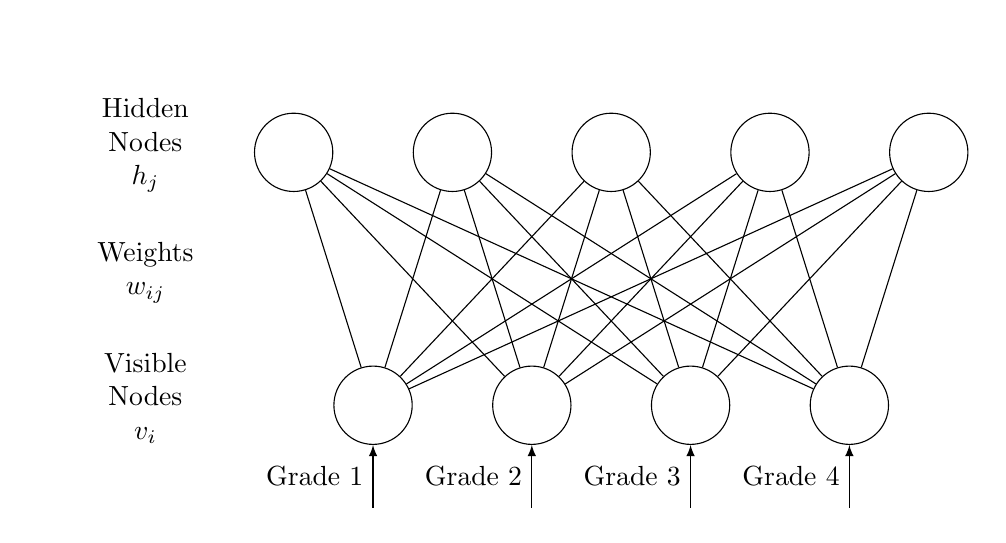
\begin{tikzpicture}[
plain/.style={
  draw=none,
  fill=none,
  },
net/.style={
  matrix of nodes,
  nodes={
    draw,
    circle,
    inner sep=10pt
    },
  nodes in empty cells,
  column sep=0pt,
  row sep=-1cm
  },
>=latex
]

\matrix[net] (mat)
{
|[plain]| \parbox{1.3cm}{\centering Hidden Nodes $h_j$} & & 
    |[plain]| & & |[plain]| & & |[plain]| & & |[plain]| & \\
|[plain]| \parbox{1.3cm}{\centering Weights $w_{ij}$}
    &|[plain]| &|[plain]| &|[plain]| &|[plain]| &
    |[plain]| &|[plain]| &|[plain]| &|[plain]| &|[plain]| \\
|[plain]| \parbox{1.3cm}{\centering Visible Nodes $v_i$} & 
    |[plain]| & & |[plain]| & & |[plain]| & & |[plain]| &\\
};
\foreach \ai [count=\mi ]in {3,5,7,9}
  \draw[<-] (mat-3-\ai) -- node[left] {Grade \mi} +(0cm,-1.3);
\foreach \ai in {2,4,...,10}
{\foreach \aii in {3,5,7,9}
  \draw[-] (mat-1-\ai) -- (mat-3-\aii);
}
\end{tikzpicture}

\caption{\label{fig:RBM}
A restricted Boltzmann machine (RBM) with 4 courses and 5 hidden
nodes for a specific student.
}
\end{figure}

Suppose the graph have $N$ visible nodes and $M$ hidden nodes,
with each visible node denoted $v_i$, hidden nodes denoted $h_j$, 
weights between two nodes $w_{ij}$,
$b_i$ and $a_j$ be bias parameters,
and $\sigma_i$ be the standard deviation of grades for each course.
Here each visible node $v_i$ represents the grade for course $i$,
where a specific student is fixed.
Let $\theta = \{ w_{ij},a_j,b_i,\sigma_i \} \; \forall i,j$,
$\mathbf{v} = \{v_i\} \; \forall i$,
and $\mathbf{h} = \{h_j\} \; \forall j$ denote the collections.
Additionally, we let the hidden nodes only take on binary values, 
i.e. $v_i \in \mathbb{R}, h_j \in \{0,1\}$.
We can then define the energy function and 
the joint distribution for the graph:
%
\begin{equation}
\begin{aligned}
    E(\mathbf{v},\mathbf{h}|\theta) &= 
        \displaystyle\sum_{i=1}^N \frac{(b_i - v_i)^2}{2 \sigma_i}
        - \displaystyle\sum_{i=1}^N \displaystyle\sum_{j=1}^M
             w_{ij} h_j \frac{v_i}{\sigma_i}
        - \displaystyle\sum_{i=j}^M a_j h_j \\
% \end{equation}
%
% The joint distribution for the graph is then defined
% by the Boltzmann distribution:
%
% \begin{equation}
    P(\mathbf{v},\mathbf{h}|\theta) &= 
        \frac{\exp\left[-E(\mathbf{v},\mathbf{h}|\theta)\right]}
        {\mathcal{Z}}
\end{aligned}
\end{equation}
%
where $\mathcal{Z}$ is the partition function normalizing
the distribution.
After marginalizing over the hidden nodes $\mathbf{h}$, 
we can find the gradient of the likelihood function
with respect to the parameters $\theta$
to perform steepest descent optimization.
Finding the gradient requires the use of Gibbs sampling,
although \cite{SaMnHi07} showed the approximate gradient
after very few iterations of Gibbs sampling is sufficient 
for optimization.

\begin{equation}
    \frac{\de P(\mathbf{v}|\theta)}{\de w_{ij}} = 
        \mathbf{E}_{\text{data}} (v_i h_j) -
        \mathbf{E}_{\text{model}} (v_i h_j)
\end{equation}

where $\mathbf{E}_{\text{data}}$ refers to expectation 
of observing the case within data,
and $\mathbf{E}_{\text{model}}$ is the expectation of 
the current model with parameters $\theta$.
Instead of using Gibbs sampling until convergence to find 
$\mathbf{E}_{\text{model}}$, 
\cite{SaMnHi07} uses $k$ iterations for a very good approximation
of the gradient.
This method is referred to contrastive divergence (CD) by the 
authors in \cite{SaMnHi07}, where CD-$k$ refers to $k$ iterations
used in Gibbs sampling.
As a result, we have a very good algorithm optimize the
RBM for likelihood.

To perform inference on a missing grade value,
one simply include an additional ``visible'' node $v_p$,
where the value is not known, 
but can be determined by the energy function:
%
\begin{equation}
\begin{aligned}
    P(v_p|\mathbf{v}) &\propto
        \displaystyle\sum_{\mathbf{h}} 
        \exp[-E(v_p,\mathbf{v},\mathbf{h})] \\
    &= \prod_{j=1}^M \left( 1 + 
        \exp\left[\sum_{i=1}^N w_{ij} v_i\right]
        \right)
\end{aligned}
\end{equation}












\section{Denoising Autoencoders} \label{sc:dae}

\paragraph{}
Another approach to unsupervised learning is using autoencoders (AEs), 
specifically in this case we will introduce the 
denoising autoencoders (DAEs) in \cite{VLLBM10}.
The autoencoder is a compression model of input data, 
such that a high dimensional input can be encoded as 
a low dimensional representation,
where the data can be reconstructed from the representation 
using a decoder.

For this problem we consider a dataset 
$\mathcal{D} = \{\mathbf{x}^{[n]}\}, 
\mathbf{x}^{[n]} \in \mathbb{R}^{N_{in}},
n \in \mathbb{N}$,
with only $\mathbf{x}$ as the input.
We also define a desired feature $\mathbf{h} \in \mathbb{R}^{N_{feat}} $
with $N_{feat} < N_{in}$,
and an encoder-decoder pair 
$f(\mathbf{x},\mathbf{w}^{(1)}), g(\mathbf{h},\mathbf{w}^{(2)})$
such that the reconstruction 
$\hat{\mathbf{x}} = g \circ f(\mathbf{x}) \approx \mathbf{x}$.
This results in a forced compression of input $\mathbf{x}$ 
into lower dimensional $\mathbf{h}$,
and in the process, the parameterization $\mathbf{w}$ retains 
further information about the data structure.

\def\layersep{2.5cm}
\begin{figure}[h]
\centering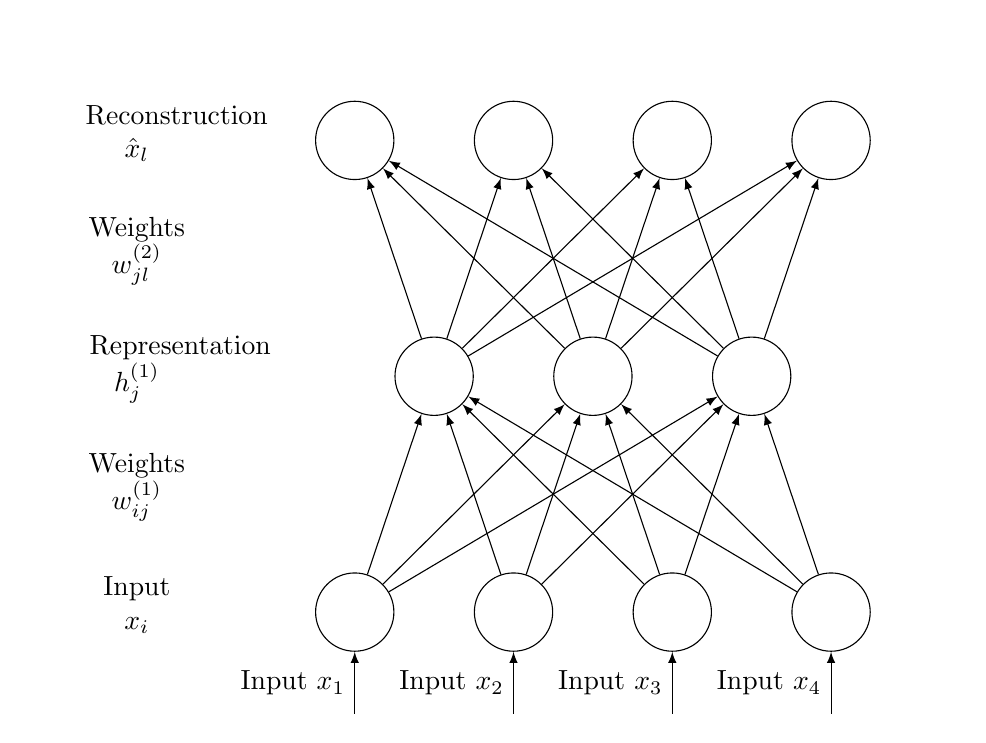
\begin{tikzpicture}[
plain/.style={
  draw=none,
  fill=none,
  },
net/.style={
  matrix of nodes,
  nodes={
    draw,
    circle,
    inner sep=10pt
    },
  nodes in empty cells,
  column sep=0pt,
  row sep=-1cm
  },
>=latex
]

\matrix[net] (mat)
{
|[plain]| \parbox{1.3cm}{\centering Reconstruction\\$\hat{x}_l$} & 
    |[plain]| & & |[plain]| & & |[plain]| & & |[plain]| &\\
% |[plain]| \parbox{1.3cm}{\centering Weights \\$w_{kl}^{(3)}$}\\
%     % &|[plain]| &|[plain]| &|[plain]| &|[plain]| &
%     % |[plain]| &|[plain]| &|[plain]| &|[plain]| &|[plain]| \\
% |[plain]| \parbox{1.2cm}{\centering Hidden\\$h_k^{(2)}$} & & 
%     |[plain]| & & |[plain]| & & |[plain]| & & |[plain]| & \\
|[plain]| \parbox{1.3cm}{\centering Weights \\$w_{jl}^{(2)}$}
    &|[plain]| &|[plain]| &|[plain]| &|[plain]| &
    |[plain]| &|[plain]| &|[plain]| &|[plain]| &|[plain]| \\
|[plain]| \parbox{1.2cm}{\centering Representation\\$h_j^{(1)}$} & |[plain]| & 
    |[plain]| & & |[plain]| & & |[plain]| & & |[plain]| & |[plain]| \\
|[plain]| \parbox{1.3cm}{\centering Weights \\$w_{ij}^{(1)}$}
    &|[plain]| &|[plain]| &|[plain]| &|[plain]| &
    |[plain]| &|[plain]| &|[plain]| &|[plain]| &|[plain]| \\
|[plain]| \parbox{1.3cm}{\centering Input\\$x_i$} & 
    |[plain]| & & |[plain]| & & |[plain]| & & |[plain]| &\\
};
\foreach \ai [count=\mi ]in {3,5,7,9}
  \draw[<-] (mat-5-\ai) -- node[left] {Input $x_\text{\mi}$} +(0cm,-1.3);
\foreach \ai in {3,5,7,9}
{\foreach \aii in {4,6,8}
  \draw[<-] (mat-1-\ai) -- (mat-3-\aii);
}
\foreach \ai in {4,6,8}
{\foreach \aii in {3,5,7,9}
  \draw[<-] (mat-3-\ai) -- (mat-5-\aii);
}
\end{tikzpicture}

\caption{\label{fig:AE1}
An one layer autoencoder with 4 input nodes and 3 representation nodes.
}
\end{figure}

With this setup, we have a neural network described as in Figure \ref{fig:AE1}.
In this structure, we can optimize for the optimal parameters 
$\{\mathbf{w}^{(1)}, \mathbf{w}^{(2)}\}$ using the gradient descent approach
from feedforward neural networks \ref{sc:nnet}. 
In practice, tied weights condition
$\mathbf{w}^{(1)} = [\mathbf{w}^{(2)}]^\top$ 
is often enforced to start the optimization.
Observe that when the weights are tied and 
the non-linear activation function is sigmoid, 
we have a striking similarity with the RBM:
the representation $\mathbf{h}$ is exactly 
the probability of binary hidden layer sampled as 1.

However as \cite{VLLBM10} explained, 
pure compression retains insufficient information,
especially when compared to RBMs;
therefore the authors introduced a new optimization criterion:
reconstruction from noisy inputs.
Formally, we have a corruption function $q$ 
that creates noisy inputs $\mathbf{v} = q(\mathbf{x})$.
A popular choice of $q$ is to randomly 
set a fraction of the input dimensions to zero.

To motivate denoising autoencoders, 
we consider an example with 2 inputs, i.e. $\mathbf{x} = \{x_1, x_2\}$,
and let $x_1 \approx \phi(x_2)$ for some bijection $\phi$.
When $x_1$ is set to zero due to corruption, 
it remains possible to reconstruct $x_1$ by 
learning the relationship between $x_1$ and $x_2$,
which gives us $\hat{x}_1 = \phi(x_2)$.
Similarly, when $x_2$ is corrupted, ideally we can have 
$\hat{x}_2 = \phi^{-1}(x_1)$.


\def\layersep{2.5cm}
\begin{figure}[h]
\centering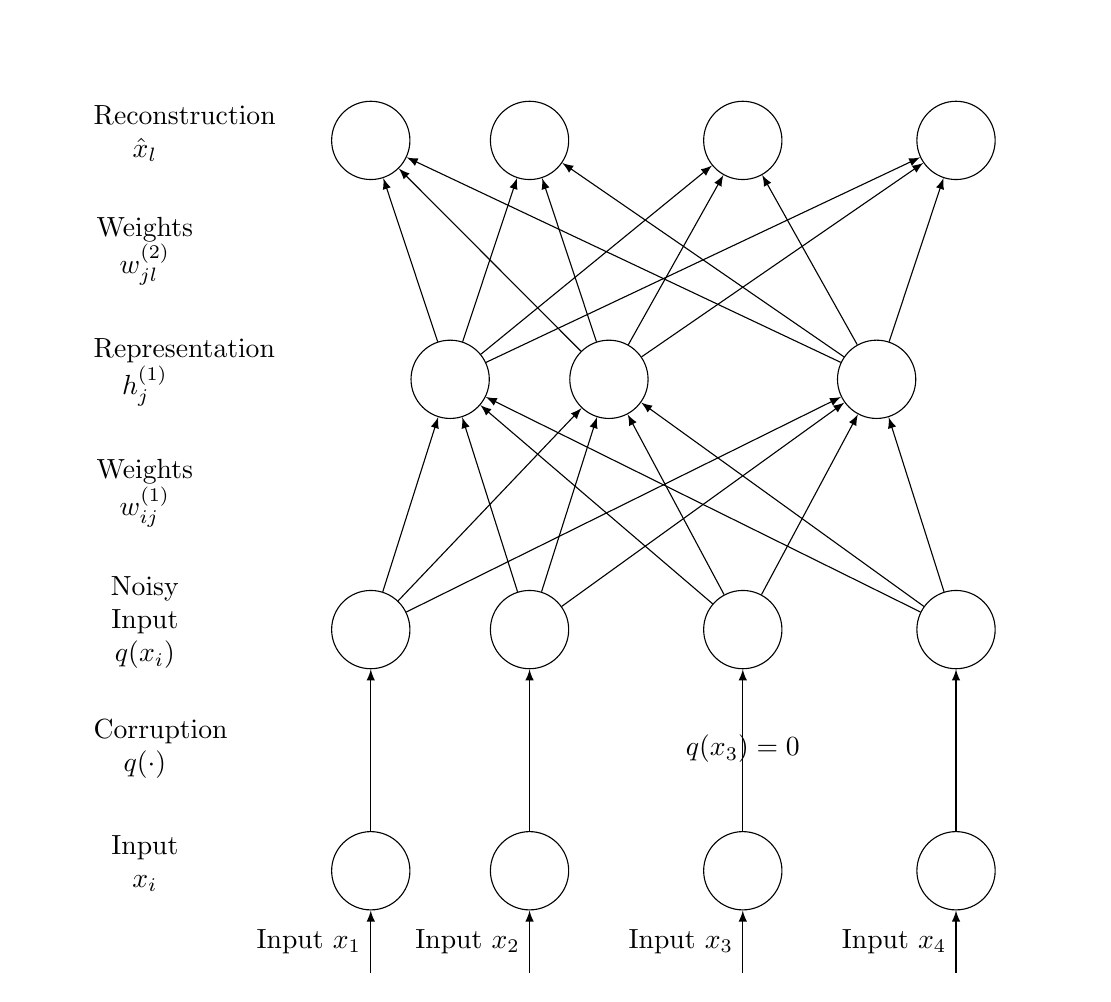
\begin{tikzpicture}[
plain/.style={
  draw=none,
  fill=none,
  },
net/.style={
  matrix of nodes,
  nodes={
    draw,
    circle,
    inner sep=10pt
    },
  nodes in empty cells,
  column sep=0pt,
  row sep=-1cm
  },
>=latex
]

\matrix[net] (mat)
{
|[plain]| \parbox{1.3cm}{\centering Reconstruction\\$\hat{x}_l$} & 
    |[plain]| & & |[plain]| & & |[plain]| & & |[plain]| &\\
|[plain]| \parbox{1.3cm}{\centering Weights \\$w_{jl}^{(2)}$}
    &|[plain]| &|[plain]| &|[plain]| &|[plain]| &
    |[plain]| &|[plain]| &|[plain]| &|[plain]| &|[plain]| \\
|[plain]| \parbox{1.3cm}{\centering Representation\\$h_j^{(1)}$} & |[plain]| & 
    |[plain]| & & |[plain]| & & |[plain]| & & |[plain]| & |[plain]| \\
|[plain]| \parbox{1.3cm}{\centering Weights \\$w_{ij}^{(1)}$}
    &|[plain]| &|[plain]| &|[plain]| &|[plain]| &
    |[plain]| &|[plain]| &|[plain]| &|[plain]| &|[plain]| \\
|[plain]| \parbox{1.3cm}{\centering Noisy Input\\$q(x_i)$} & 
    |[plain]| & & |[plain]| & & |[plain]| & & |[plain]| &\\
|[plain]| \parbox{1.3cm}{\centering Corruption \\$q(\cdot)$}
    &|[plain]| &|[plain]| &|[plain]| &|[plain]| &
    |[plain]| & |[plain]| $q(x_3)=0$ &|[plain]| &|[plain]| &|[plain]| \\
|[plain]| \parbox{1.3cm}{\centering Input\\$x_i$} & 
    |[plain]| & & |[plain]| & & |[plain]| & & |[plain]| &\\
};
\foreach \ai [count=\mi ]in {3,5,7,9}
  \draw[<-] (mat-7-\ai) -- node[left] {Input $x_\text{\mi}$} +(0cm,-1.3);
\foreach \ai in {3,5,7,9}
  \draw[<-] (mat-5-\ai) -- (mat-7-\ai);
% \draw[<-] (mat-5-7) -- node[left] {$q(x_3) = 0$} +(0cm,-2.8cm);
\foreach \ai in {3,5,7,9}
{\foreach \aii in {4,6,8}
  \draw[<-] (mat-1-\ai) -- (mat-3-\aii);
}
\foreach \ai in {4,6,8}
{\foreach \aii in {3,5,7,9}
  \draw[<-] (mat-3-\ai) -- (mat-5-\aii);
}
\end{tikzpicture}

\caption{\label{fig:DAE1}
An one layer denoising autoencoder with 4 input nodes, 3 representation nodes,
and symmetric weights. In this case, we have the third input corrupted
by setting to zero.
}
\end{figure}

























\section{MNIST Hand-Written Digits Example} \label{sc:MNIST}

\paragraph{}
The Mixed National Institute of Standards and Technology
(MNIST) dataset \cite{Le98} is a collection of images of hand-written digits
from various sources,
with each image labeled the correct digit.
The dataset contains 60,000 images for training (fitting),
and 10,000 images for testing.
The images are 28x28 in resolution,
hence making $N^{(1)} = 784$ dimensions in input.

The data labels are changed to use the 1-of-K encoding scheme,
where the label $\mathbf{y}$ is a binary vector of size K,
with only one element taking a value of one.
In this case, given 10 possible digits,
we have a vector of size $N^{(4)} = 10$.
For example, a possible scheme can label the digit ``$3$'' 
using the vector $[0,0,1,0,\ldots]$ where 
only the $3^\text{rd}$ index is a ``$1$''.

To best model this type of label vector,
the softmax function is chosen for the output layer:
%
\begin{equation*}
	f_l = 
	g^{(3)}(z_l^{(3)}) = \frac{\exp(z_l^{(3)})}
		{\sum_{k=1}^{N^{(4)}} \exp(z_k^{(3)})}
\end{equation*}
%
where $z^{(3)}_l = \sum_{k=1}^{N^{(3)}} w_{kl}^{(3)} h_k^{(2)} + 
      w^{(3)}_{0l}$ 
      is a linear combination of the final hidden layer.
Since the denominator normalizes the sum, the $f_l$ now adds up to one,
and a ``perfect'' output is exactly the 1-of-K encoded label.
If $f_l$ is modeled as the probability of the image being digit $l$,
suppose the correct digit is $m$,
then the likelihood of making the correct prediction is:
%
\begin{equation*}
  L(\mathbf{f},\mathbf{y}) = f_m = \prod_{l=1}^{N^{(4)}} f_l \, ^{y_l}
\end{equation*}
%
since $y_m = 1$ is the only non-zero term in the label vector.
We can then define the error function as negative log-likelihood:
%
\begin{equation*}
% \begin{aligned}
	E(\mathbf{f},\mathbf{y}) 
		= - \log \prod_{l=1}^{N^{(4)}} f_l \, ^{y_l}
		= - \sum_{l=1}^{N^{(4)}} y_l \log f_l
% \end{aligned}
\end{equation*}
%
where $N^{(4)}$ is the number of output nodes, 
and minimizing $E$ is equivalent to maximizing likelihood.
Note taking the logarithm creates an error function with much
simpler derivative, 
hence simplifying the gradient descent method.

In the following experiment, 
a two hidden layer neural network is used to model the MNIST digits.
We used $N^{(2)} = N^{(3)} = 1000$ nodes in the hidden layers, 
creating a structure of 784-1000-1000-10 
$\left( N^{(1)} - N^{(2)} - N^{(3)} - N^{(4)} \right)$
nodes in each layer.
We also chose 
$g^{(1)}(\cdot) = g^{(2)}(\cdot) = g_\text{ReLU}(\cdot)$ 
in the hidden layers,
and softmax for the output layer.
The hyper parameters were chosen as $\eta = 10^{-5}$
and $\theta = 0.9$.
We also chose to update the weight vector $\mathbf{w}^k$ once
for every 100 samples of digits,
also known as a mini-batch.

After training (optimizing) for 50 epochs,
with each epoch denoting one complete run through of the training 
dataset,
we reach a test error rate of $16\%$ (Figure \ref{fig:mnist_err}).
%
\begin{figure}[h]
\centering
\begin{subfigure}{.45\textwidth}
  \centering
  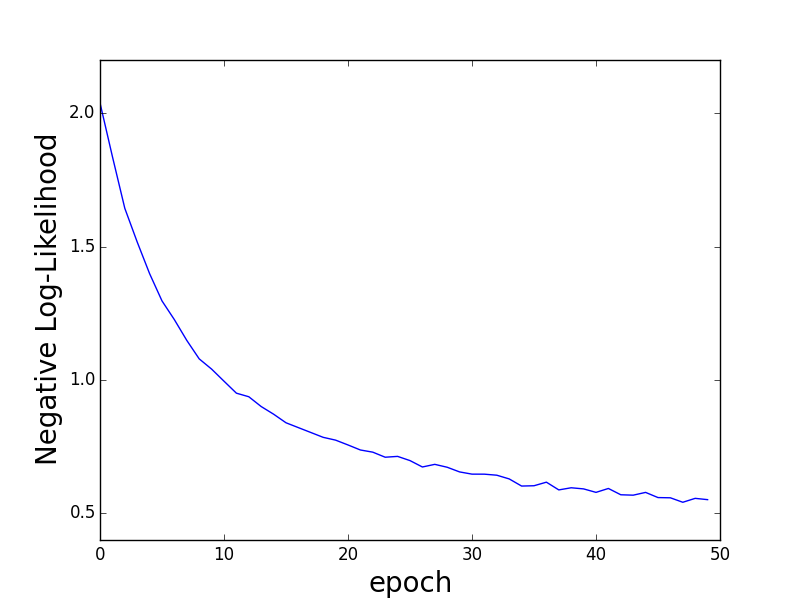
\includegraphics[width=\linewidth]{fig_mnist_nll.png}
  \caption{The negative log-likelihood}
  \label{fig:mnist_nll}
\end{subfigure}%
\begin{subfigure}{.45\textwidth}
  \centering
  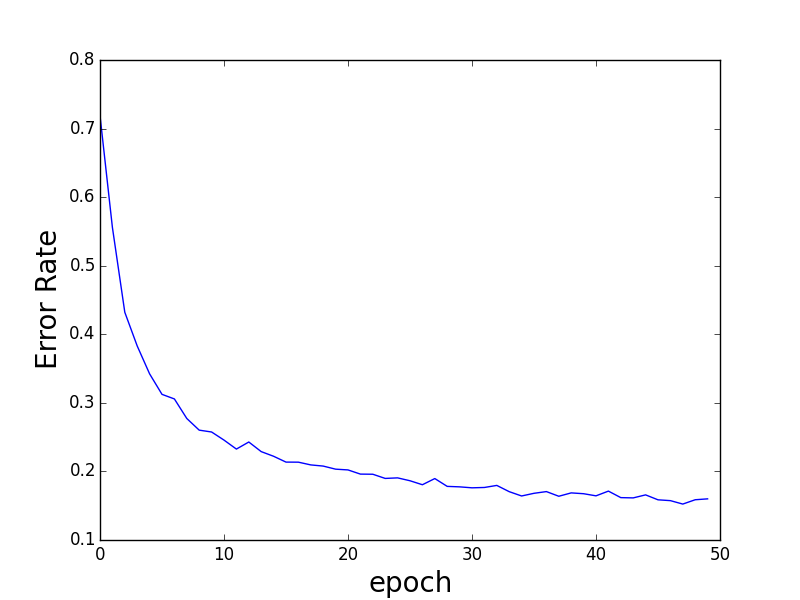
\includegraphics[width=\linewidth]{fig_mnist_err.png}
  \caption{The classification error rate}
  \label{fig:mnist_err}
\end{subfigure}
\caption{MNIST hand-written digits modeled using a two hidden
  layer neural network, with negative log-likelihood and
  classification error rate computed after each epoch.}
\label{fig:mnist_results}
\end{figure}
%
By increasing the number of epochs and a few minor modifications,
this model could potentially reach error rates as low as $2\%$.
However, this will not be explored since it is not
the main purpose of this document,
and optimization can be very time consuming due to computation.

% It is important to note that the activation function chosen is ReLU, 
% which is not easy to incorporate due within a 
% restricted Boltzmann machine context due to an unbounded range.
% However, a recently introduced method called 
% general adversarial networks can be used instead using the ReLU functions
% in alternative to restricted Boltzmann machines.
% This will be explored further in future discussions.

While the technique is more than a sufficient solution 
for recognizing hand-written digits,
naively applying gradient descent to more complex 
neural networks tend to have poor results.
Alternative methods will be discussed in the next section 
in order to address this problem.

Also note this type of neural networks is feed-forward, 
which mean it is limited to only supervised type problems
where the data structure is consistent 
and a prediction target (label) is provided for each sample.
For a collaborative filtering type problem,
the inference is often made within the data structure itself, 
which makes an unsupervised learning problem.
Feed-forward neural networks also fail to fully utilize 
the datasets that are partly labeled, 
known as semi-supervised problems.
These problems would require other variations of neural networks
with different methods for inference.







\chapter{Unsupervised Learning} \label{ch:unsupervised_learning}

\section{Restricted Boltzmann Machines} \label{sc:rbm}

\paragraph{}
On the other hand, restricted Boltzmann machines (RBM) is a
completely different approach to problems without labels.
RBM is a type of unsupervised learning algorithm, 
for there are no labels to ``supervise'' the learning.
The purpose of unsupervised algorithms are to find
structural patterns within the data itself.
In this case, we are interested in the relationships 
between the performance in difference courses,
and how this helps us predict the grades.

A RBM is a Markov random field in the form of a bipartite graph,
where the joint probability follows a Boltzmann type distribution.
The bipartite graph structure creates two layers without
internal connections.
One layer, called the visible layer, contain the input data; 
in this case, the visible values are the grades of each student.
These nodes are connected to the other layer, called the hidden layer,
with symmetrical weighted connections.
%
\def\layersep{2.5cm}
\begin{figure}[h]
\centering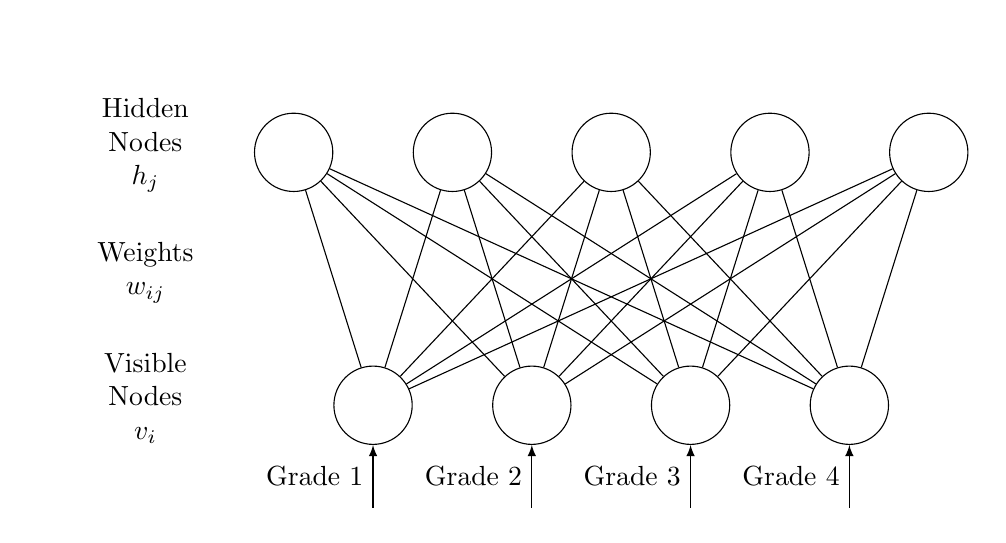
\begin{tikzpicture}[
plain/.style={
  draw=none,
  fill=none,
  },
net/.style={
  matrix of nodes,
  nodes={
    draw,
    circle,
    inner sep=10pt
    },
  nodes in empty cells,
  column sep=0pt,
  row sep=-1cm
  },
>=latex
]

\matrix[net] (mat)
{
|[plain]| \parbox{1.3cm}{\centering Hidden Nodes $h_j$} & & 
    |[plain]| & & |[plain]| & & |[plain]| & & |[plain]| & \\
|[plain]| \parbox{1.3cm}{\centering Weights $w_{ij}$}
    &|[plain]| &|[plain]| &|[plain]| &|[plain]| &
    |[plain]| &|[plain]| &|[plain]| &|[plain]| &|[plain]| \\
|[plain]| \parbox{1.3cm}{\centering Visible Nodes $v_i$} & 
    |[plain]| & & |[plain]| & & |[plain]| & & |[plain]| &\\
};
\foreach \ai [count=\mi ]in {3,5,7,9}
  \draw[<-] (mat-3-\ai) -- node[left] {Grade \mi} +(0cm,-1.3);
\foreach \ai in {2,4,...,10}
{\foreach \aii in {3,5,7,9}
  \draw[-] (mat-1-\ai) -- (mat-3-\aii);
}
\end{tikzpicture}

\caption{\label{fig:RBM}
A restricted Boltzmann machine (RBM) with 4 courses and 5 hidden
nodes for a specific student.
}
\end{figure}

Suppose the graph have $N$ visible nodes and $M$ hidden nodes,
with each visible node denoted $v_i$, hidden nodes denoted $h_j$, 
weights between two nodes $w_{ij}$,
$b_i$ and $a_j$ be bias parameters,
and $\sigma_i$ be the standard deviation of grades for each course.
Here each visible node $v_i$ represents the grade for course $i$,
where a specific student is fixed.
Let $\theta = \{ w_{ij},a_j,b_i,\sigma_i \} \; \forall i,j$,
$\mathbf{v} = \{v_i\} \; \forall i$,
and $\mathbf{h} = \{h_j\} \; \forall j$ denote the collections.
Additionally, we let the hidden nodes only take on binary values, 
i.e. $v_i \in \mathbb{R}, h_j \in \{0,1\}$.
We can then define the energy function and 
the joint distribution for the graph:
%
\begin{equation*}
\begin{aligned}
    E(\mathbf{v},\mathbf{h}|\theta) &= 
        \displaystyle\sum_{i=1}^N \frac{(b_i - v_i)^2}{2 \sigma_i}
        - \displaystyle\sum_{i=1}^N \displaystyle\sum_{j=1}^M
             w_{ij} h_j \frac{v_i}{\sigma_i}
        - \displaystyle\sum_{i=j}^M a_j h_j \\
% \end{equation*}
%
% The joint distribution for the graph is then defined
% by the Boltzmann distribution:
%
% \begin{equation*}
    P(\mathbf{v},\mathbf{h}|\theta) &= 
        \frac{\exp\left[-E(\mathbf{v},\mathbf{h}|\theta)\right]}
        {\mathcal{Z}}
\end{aligned}
\end{equation*}
%
where $\mathcal{Z}$ is the partition function normalizing
the distribution.
After marginalizing over the hidden nodes $\mathbf{h}$, 
we can find the gradient of the likelihood function
with respect to the parameters $\theta$
to perform steepest descent optimization.
Finding the gradient requires the use of Gibbs sampling,
although \cite{SaMnHi07} showed the approximate gradient
after very few iterations of Gibbs sampling is sufficient 
for optimization.

\begin{equation*}
    \frac{\de P(\mathbf{v}|\theta)}{\de w_{ij}} = 
        \mathbf{E}_{\text{data}} (v_i h_j) -
        \mathbf{E}_{\text{model}} (v_i h_j)
\end{equation*}

where $\mathbf{E}_{\text{data}}$ refers to expectation 
of observing the case within data,
and $\mathbf{E}_{\text{model}}$ is the expectation of 
the current model with parameters $\theta$.
Instead of using Gibbs sampling until convergence to find 
$\mathbf{E}_{\text{model}}$, 
\cite{SaMnHi07} uses $k$ iterations for a very good approximation
of the gradient.
This method is referred to contrastive divergence (CD) by the 
authors in \cite{SaMnHi07}, where CD-$k$ refers to $k$ iterations
used in Gibbs sampling.
As a result, we have a very good algorithm optimize the
RBM for likelihood.

To perform inference on a missing grade value,
one simply include an additional ``visible'' node $v_p$,
where the value is not known, 
but can be determined by the energy function:
%
\begin{equation*}
\begin{aligned}
    P(v_p|\mathbf{v}) &\propto
        \displaystyle\sum_{\mathbf{h}} 
        \exp[-E(v_p,\mathbf{v},\mathbf{h})] \\
    &= \prod_{j=1}^M \left( 1 + 
        \exp\left[\sum_{i=1}^N w_{ij} v_i\right]
        \right)
\end{aligned}
\end{equation*}












\section{Denoising Autoencoders} \label{sc:dae}

\paragraph{}
Another approach to unsupervised learning is using autoencoders (AEs), 
specifically in this case we will introduce the 
denoising autoencoders (DAEs) in \cite{VLLBM10}.
The autoencoder is a compression model of input data, 
such that a high dimensional input can be encoded as 
a low dimensional representation,
where the data can be reconstructed from the representation 
using a decoder.

For this problem we consider a dataset 
$\mathcal{D} = \{\mathbf{x}^{[n]}\}, 
\mathbf{x}^{[n]} \in \mathbb{R}^{N_{in}},
n \in \mathbb{N}$,
with only $\mathbf{x}$ as the input.
We also define a desired feature $\mathbf{h} \in \mathbb{R}^{N_{feat}} $
with $N_{feat} < N_{in}$,
and an encoder-decoder pair 
$f(\mathbf{x},\mathbf{w}^{(1)}), g(\mathbf{h},\mathbf{w}^{(2)})$
such that the reconstruction 
$\hat{\mathbf{x}} = g \circ f(\mathbf{x}) \approx \mathbf{x}$.
This results in a forced compression of input $\mathbf{x}$ 
into lower dimensional $\mathbf{h}$,
and in the process, the parameterization $\mathbf{w}$ retains 
further information about the data structure.

\def\layersep{2.5cm}
\begin{figure}[H]
\centering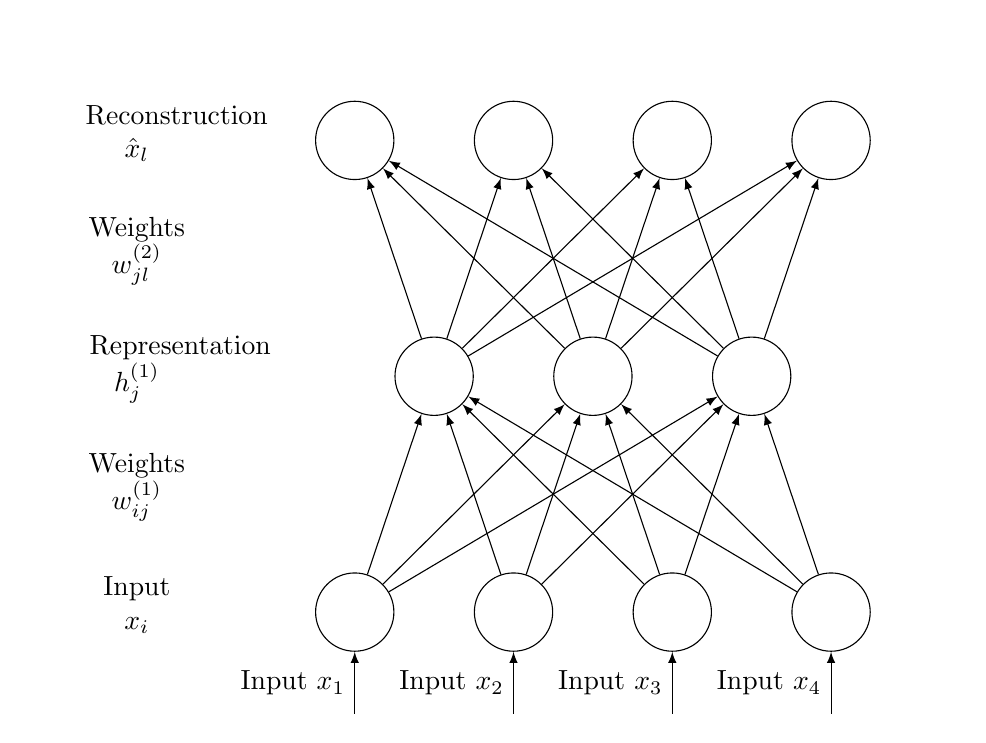
\begin{tikzpicture}[
plain/.style={
  draw=none,
  fill=none,
  },
net/.style={
  matrix of nodes,
  nodes={
    draw,
    circle,
    inner sep=10pt
    },
  nodes in empty cells,
  column sep=0pt,
  row sep=-1cm
  },
>=latex
]

\matrix[net] (mat)
{
|[plain]| \parbox{1.3cm}{\centering Reconstruction\\$\hat{x}_l$} & 
    |[plain]| & & |[plain]| & & |[plain]| & & |[plain]| &\\
% |[plain]| \parbox{1.3cm}{\centering Weights \\$w_{kl}^{(3)}$}\\
%     % &|[plain]| &|[plain]| &|[plain]| &|[plain]| &
%     % |[plain]| &|[plain]| &|[plain]| &|[plain]| &|[plain]| \\
% |[plain]| \parbox{1.2cm}{\centering Hidden\\$h_k^{(2)}$} & & 
%     |[plain]| & & |[plain]| & & |[plain]| & & |[plain]| & \\
|[plain]| \parbox{1.3cm}{\centering Weights \\$w_{jl}^{(2)}$}
    &|[plain]| &|[plain]| &|[plain]| &|[plain]| &
    |[plain]| &|[plain]| &|[plain]| &|[plain]| &|[plain]| \\
|[plain]| \parbox{1.2cm}{\centering Representation\\$h_j^{(1)}$} & |[plain]| & 
    |[plain]| & & |[plain]| & & |[plain]| & & |[plain]| & |[plain]| \\
|[plain]| \parbox{1.3cm}{\centering Weights \\$w_{ij}^{(1)}$}
    &|[plain]| &|[plain]| &|[plain]| &|[plain]| &
    |[plain]| &|[plain]| &|[plain]| &|[plain]| &|[plain]| \\
|[plain]| \parbox{1.3cm}{\centering Input\\$x_i$} & 
    |[plain]| & & |[plain]| & & |[plain]| & & |[plain]| &\\
};
\foreach \ai [count=\mi ]in {3,5,7,9}
  \draw[<-] (mat-5-\ai) -- node[left] {Input $x_\text{\mi}$} +(0cm,-1.3);
\foreach \ai in {3,5,7,9}
{\foreach \aii in {4,6,8}
  \draw[<-] (mat-1-\ai) -- (mat-3-\aii);
}
\foreach \ai in {4,6,8}
{\foreach \aii in {3,5,7,9}
  \draw[<-] (mat-3-\ai) -- (mat-5-\aii);
}
\end{tikzpicture}

\caption{\label{fig:AE1}
An one layer autoencoder with 4 input nodes and 3 representation nodes.
}
\end{figure}

With this setup, we have a neural network described as in Figure \ref{fig:AE1}.
In this structure, we can optimize for the optimal parameters 
$\{\mathbf{w}^{(1)}, \mathbf{w}^{(2)}\}$ using the gradient descent approach
from feedforward neural networks \ref{sc:nnet}. 
In practice, tied weights condition
$\mathbf{w}^{(1)} = [\mathbf{w}^{(2)}]^\top$ 
is often enforced to start the optimization.
Observe that when the weights are tied and 
the non-linear activation function is sigmoid, 
we have a striking similarity with the RBM:
the representation $\mathbf{h}$ is exactly 
the probability of binary hidden layer sampled as 1.

However as \cite{VLLBM10} explained, 
pure compression retains insufficient information,
especially when compared to RBMs;
therefore the authors introduced a new optimization criterion:
reconstruction from noisy inputs.
Formally, we have a corruption function $q$ 
that creates noisy inputs $\mathbf{v} = q(\mathbf{x})$.
A popular choice of $q$ is to randomly 
set a fraction of the input dimensions to zero.

To motivate denoising autoencoders, 
we consider an example with 2 inputs, i.e. $\mathbf{x} = \{x_1, x_2\}$,
and let $x_1 \approx \phi(x_2)$ for some bijection $\phi$.
When $x_1$ is set to zero due to corruption, 
it remains possible to reconstruct $x_1$ by 
learning the relationship between $x_1$ and $x_2$,
which gives us $\hat{x}_1 = \phi(x_2)$.
Similarly, when $x_2$ is corrupted, ideally we can have 
$\hat{x}_2 = \phi^{-1}(x_1)$.


\def\layersep{2.5cm}
\begin{figure}[H]
\centering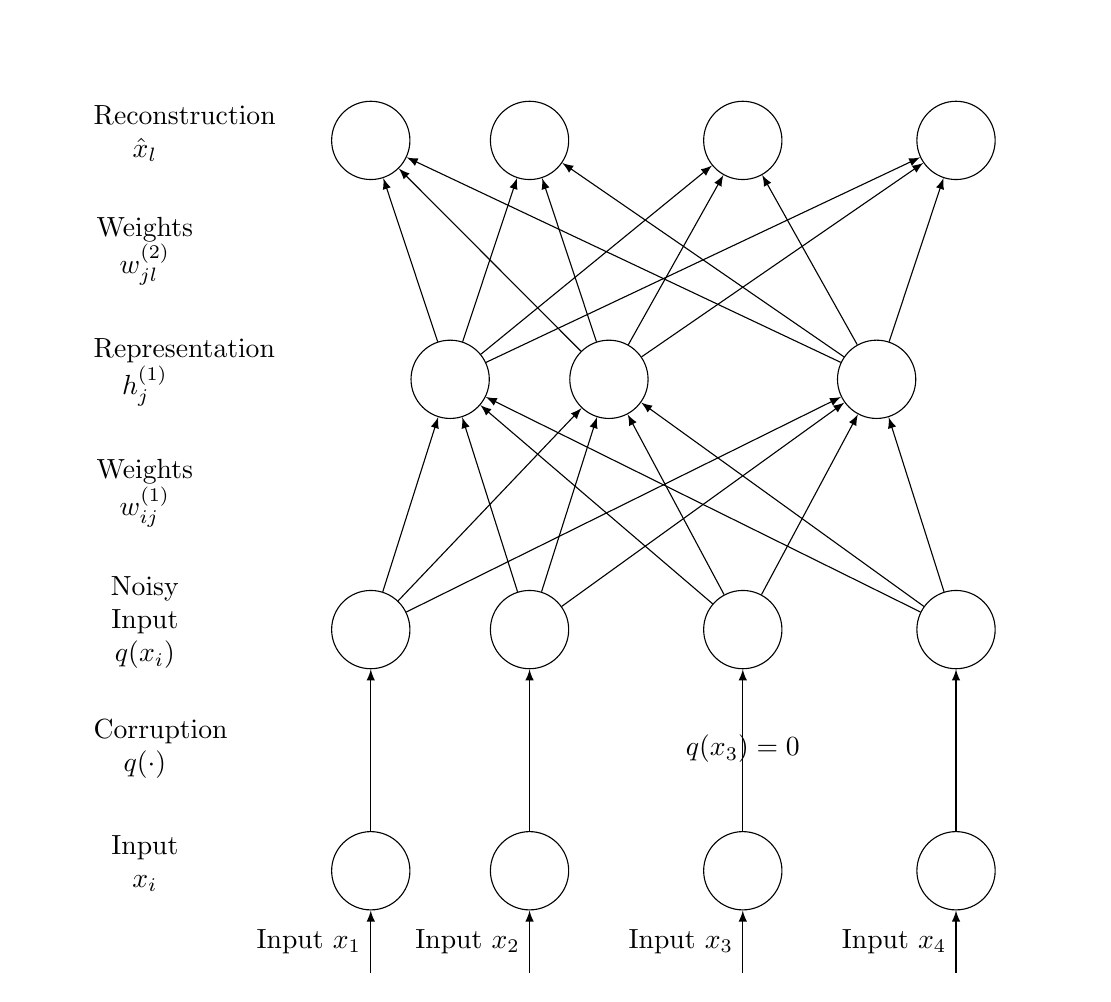
\begin{tikzpicture}[
plain/.style={
  draw=none,
  fill=none,
  },
net/.style={
  matrix of nodes,
  nodes={
    draw,
    circle,
    inner sep=10pt
    },
  nodes in empty cells,
  column sep=0pt,
  row sep=-1cm
  },
>=latex
]

\matrix[net] (mat)
{
|[plain]| \parbox{1.3cm}{\centering Reconstruction\\$\hat{x}_l$} & 
    |[plain]| & & |[plain]| & & |[plain]| & & |[plain]| &\\
|[plain]| \parbox{1.3cm}{\centering Weights \\$w_{jl}^{(2)}$}
    &|[plain]| &|[plain]| &|[plain]| &|[plain]| &
    |[plain]| &|[plain]| &|[plain]| &|[plain]| &|[plain]| \\
|[plain]| \parbox{1.3cm}{\centering Representation\\$h_j^{(1)}$} & |[plain]| & 
    |[plain]| & & |[plain]| & & |[plain]| & & |[plain]| & |[plain]| \\
|[plain]| \parbox{1.3cm}{\centering Weights \\$w_{ij}^{(1)}$}
    &|[plain]| &|[plain]| &|[plain]| &|[plain]| &
    |[plain]| &|[plain]| &|[plain]| &|[plain]| &|[plain]| \\
|[plain]| \parbox{1.3cm}{\centering Noisy Input\\$q(x_i)$} & 
    |[plain]| & & |[plain]| & & |[plain]| & & |[plain]| &\\
|[plain]| \parbox{1.3cm}{\centering Corruption \\$q(\cdot)$}
    &|[plain]| &|[plain]| &|[plain]| &|[plain]| &
    |[plain]| & |[plain]| $q(x_3)=0$ &|[plain]| &|[plain]| &|[plain]| \\
|[plain]| \parbox{1.3cm}{\centering Input\\$x_i$} & 
    |[plain]| & & |[plain]| & & |[plain]| & & |[plain]| &\\
};
\foreach \ai [count=\mi ]in {3,5,7,9}
  \draw[<-] (mat-7-\ai) -- node[left] {Input $x_\text{\mi}$} +(0cm,-1.3);
\foreach \ai in {3,5,7,9}
  \draw[<-] (mat-5-\ai) -- (mat-7-\ai);
% \draw[<-] (mat-5-7) -- node[left] {$q(x_3) = 0$} +(0cm,-2.8cm);
\foreach \ai in {3,5,7,9}
{\foreach \aii in {4,6,8}
  \draw[<-] (mat-1-\ai) -- (mat-3-\aii);
}
\foreach \ai in {4,6,8}
{\foreach \aii in {3,5,7,9}
  \draw[<-] (mat-3-\ai) -- (mat-5-\aii);
}
\end{tikzpicture}

\caption{\label{fig:DAE1}
An one layer denoising autoencoder with 4 input nodes, 3 representation nodes,
and symmetric weights. In this case, we have the third input corrupted
by setting to zero.
}
\end{figure}

\input{results}
% \input{conclusion}

%% This adds a line for the Bibliography in the Table of Contents.
\addcontentsline{toc}{chapter}{Bibliography}
%% *** Set the bibliography style. ***
%% (change according to your preference/requirements)
\bibliographystyle{plain}
%% *** Set the bibliography file. ***
%% ("thesis.bib" by default; change as needed)
\bibliography{thesis}

%% *** NOTE ***
%% If you don't use bibliography files, comment out the previous line
%% and use \begin{thebibliography}...\end{thebibliography}.  (In that
%% case, you should probably put the bibliography in a separate file and
%% `\include' or `\input' it here).

\end{document}
